\subsection{Task 1: Initial Observations on the Valve}
\label{sec:task1}

In this section, first simulations will be done on the valvular conduit. As the first ste, the sketch of the valve must be constructed. For the dimensional parameters, the optimum values of $\alpha$, $\beta$ and R are chosen so that the inner circular arc is tangent to the x-axis. A sample sketch for this geometry can be seen on Figure \ref{fig:sampsketch}.

\begin{figure}[H]
    \centering
    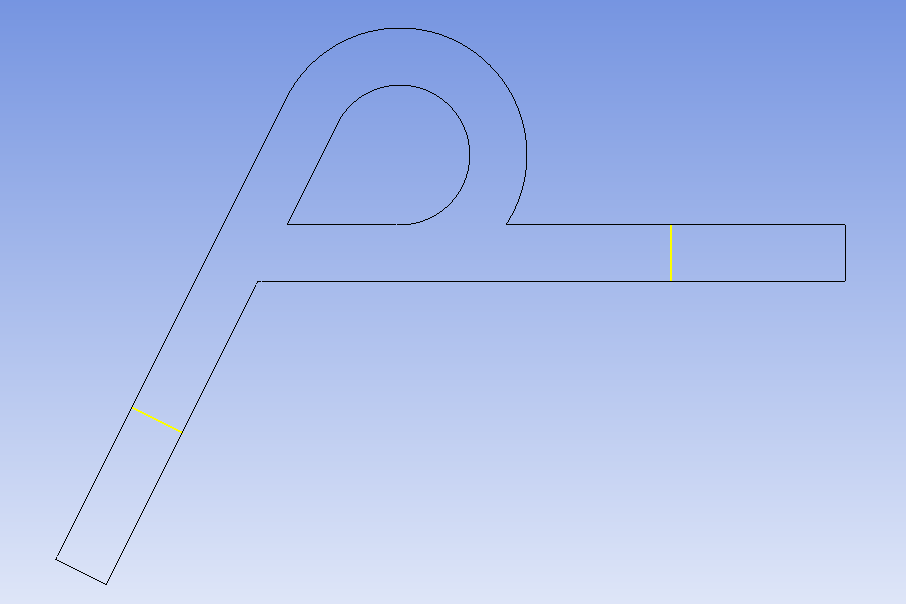
\includegraphics[width=.6\textwidth]{images/task1/data_locations.png}
    \caption{Sample Sketch}
    \label{fig:sampsketch}
\end{figure}

For this geometry, the straight line segment is selected to be 200mm long and Re is chosen to be 181. To obtain that value the velocity and material properties as manipulated as follows:
\begin{itemize}
    \item $\mu = 4.6.10^{-4}$Pa.s
    \item $\rho = 1000 kg/m^{3}$
    \item $D = 100$mm
    \item $V = 0.0008326$m/s
\end{itemize}

For the boundary conditions, no-slip on channel walls and uniform inlet velocity are set. This task only tests the forward flow throughout the inlet. To achieve this, the inlet is selected to be the end of the horizontal segment at the right-hand side of the sketch. To observe the grid-independence of the solution, two different mesh sizes are used, them being $6.10^{-3}$ and $6.10^{-3}$ meters with adaptive meshing. In order to prove that grid convergence is achieved, velocity profile of the fluid halfway through the inlet segment and outlet segment is plotted between two mesh sizes. As can be seen from Figure \ref{fig:mesh_comp}, the results does not change considerably with reducing mesh size. From this, a mesh size of $3.10^{-3}$m will be used in this project unless stated otherwise. 

\begin{figure}[H]
 \centering
\begin{subfigure}{.45\textwidth}
  \centering
  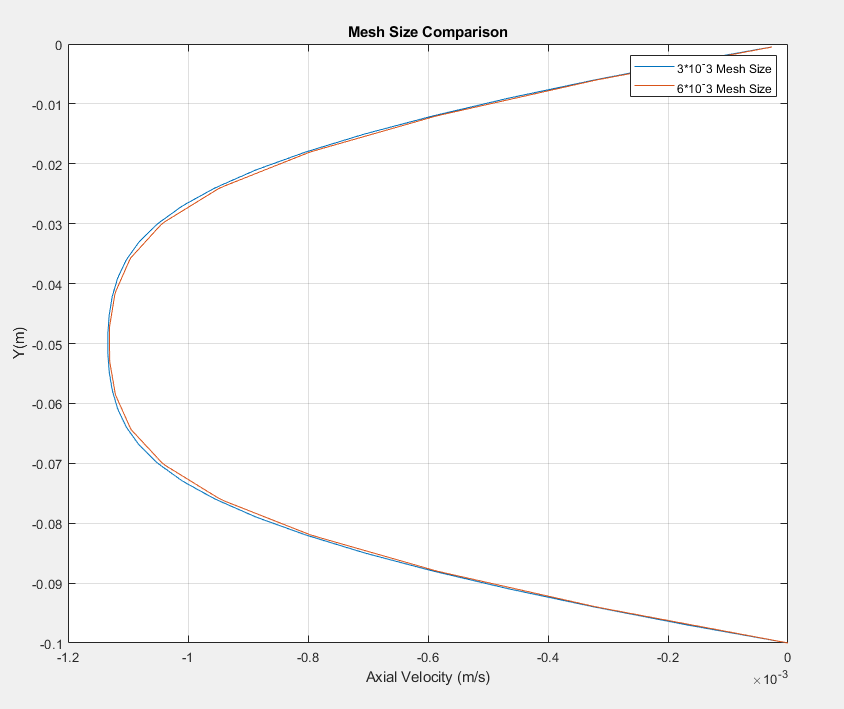
\includegraphics[width=.87\linewidth]{images/task1/3vs6mesh.png}
  \caption{Profile at the inlet}
  \label{fig:x_d_norm}
\end{subfigure}%
~
\begin{subfigure}{.45\textwidth}
  \centering
  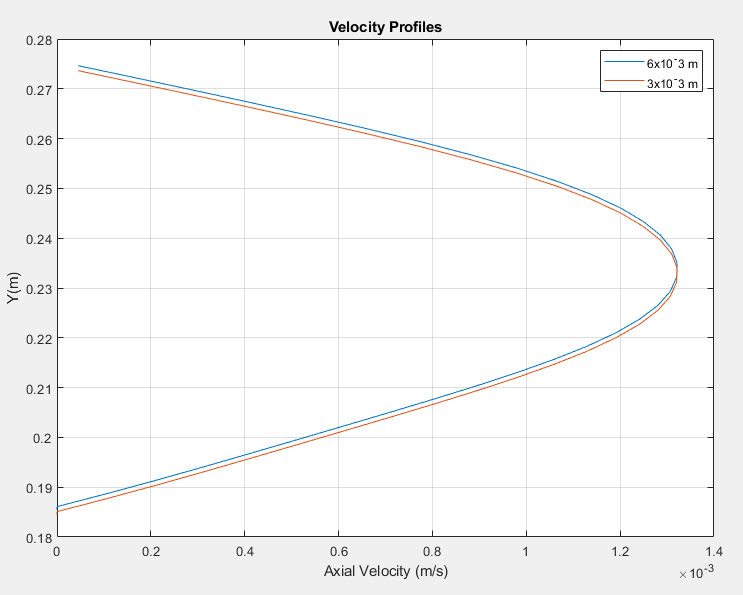
\includegraphics[width=.9\linewidth]{images/task1/outlet_mesh_comparison.png}
  \caption{Profile at the outlet}
  \label{fig:x_d_norm_actual}
\end{subfigure}
~
\caption{Mesh Size Comparison}
\label{fig:mesh_comp}
\end{figure}